% ==============================================================================================
\chapter{Moving load on a beam} \label{ch:moving_load_beam}
% ==============================================================================================

% ----------------------------------------------------------------------------------------------
\section{Introduction}
% ----------------------------------------------------------------------------------------------

This benchmark compares the STEM numerical solution against the analytical solution for the dynamic response of a
simply supported beam subjected to a moving load, traveling at a constant speed from one end of the beam to the other.

The STEM numerical response is compared with the analytical solution, presented in ~\cite[Chapter 1.3.2.2]{Fryba_1972}.
The analytical solution provides closed-form expressions for the vertical displacement along the beam, enabling a
direct time-history comparison against the numerical model.


% ----------------------------------------------------------------------------------------------
\section{Model Description}
% ----------------------------------------------------------------------------------------------

% ..............................................................................................
\subsection{Geometry and loading}
% ..............................................................................................
The model consists of a simply supported beam with a length of \qty{25}{\meter}. The beam is subjected to
a moving vertical point load with a magnitude of \qty{1}{\kilo\newton}. The load travels at a constant speed of
\qty{10}{\meter\per\second}, starting at the left support.
The analysis is performed for both 2D and 3D configurations.

Figure~\ref{fig:moving_load_on_beam_model} illustrates the geometry, boundary conditions and loading of the
simply supported beam with the moving load.

\begin{figure}
    \centering
    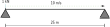
\includegraphics[width=0.8\textwidth]{moving_load_on_beam/simply_supported_beam_with_moving_load.pdf}
    \caption{Geometry, boundary conditions and loading of the simply supported beam.}
    \label{fig:moving_load_on_beam_model}
\end{figure}

% ..............................................................................................
\subsection{Materials and numerical parameters}
% ..............................................................................................
The simply supported beam is modelled using Euler-Bernoulli beam elements. The beam properties used in analysis are:

\begin{itemize}[noitemsep,topsep=0pt,parsep=0pt,partopsep=0pt]
	\item Young's modulus: \qty{210e9}{\newton\per\meter\squared},
	\item Poisson ratio: \qty{0.3}{},
	\item Density: \qty{7850}{\kilogram\per\meter\cubed},
	\item Cross-sectional area: \qty{0.01}{\meter\squared},
    \item Moment of inertia: \qty{0.0001}{\meter\tothe{4}},
\end{itemize}

The beam is discretised using beam elements with an element size of \qty{2.5}{\meter}.

The dynamic analysis has a duration of \qty{2.5}{\second} with a time step of \qty{0.0025}{\second}.
The equations of motion are integrated with the Newmark scheme~\cite{Newmark_1959} using the average
acceleration parameters $\beta = 0.25$ and $\gamma = 0.5$. No damping is considered in the analysis.

% ----------------------------------------------------------------------------------------------
\section{Results}
% ----------------------------------------------------------------------------------------------
Figure~\ref{fig:moving_load_on_beam_results} shows the vertical displacement history at the mid-span of the beam
obtained using STEM in both 2D and 3D, and compares it with the analytical solution. The results show that the
mid-span deflections obtained with STEM are in agreement
with the analytical solution.

\begin{figure}[h]
	\centering
	\includegraphics[width=0.8\textwidth]{moving_load_on_beam/moving_load_on_beam_results.pdf}
	\caption{Comparison between the STEM and analytical vertical displacement at mid-span of the simply supported beam.}
	\label{fig:moving_load_on_beam_results}
\end{figure}

